\section{Baselines}

\subsection{Baseline With langid.py}

As a baseline to compare the performance of the models in we compare with an out of the box language classification system. ``langid.py: An Off-the-shelf Language Identification Tool." \cite{langID} is such a tool.\\

Out of the box langid.py comes with with a pretrained model which covers 97 languages. The data for langid.py comes from from 5 different domains: government documents, software documentation, newswire, online encyclopedia and an internet crawl.\\

We evaluated how well langid.py performed on the Wikipedia dataset. Since langid.py returned the language id ``no" (Norwegian) on some of the data points we restrict langid.py to only be able to return either ``nn" (Nynorsk) or ``nb" (Bokmål) as predictions. It is a quite peculiar feature of the Norwegian language that there exist two different written languages but three different language codes.\\

\begin{figure}[h!]
  \centering
  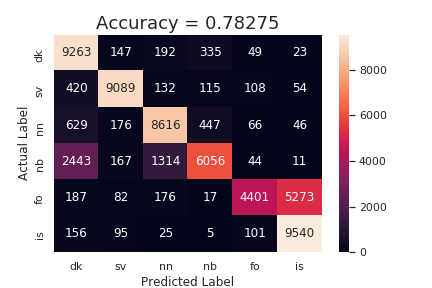
\includegraphics[width = 200pt]{figs/langid}
  \caption{Confusion matrix with results from langid.py on the full dataset with 300K data points. }
  \label{langid_confusion_matrix}
\end{figure}

In Figure~\ref{langid_confusion_matrix} we see the confusion matrix for the langid.py classifier. The largest errors are between Danish and Bokmål and between Faroese and Icelandic. We see that langid.py was actually able to correctly classify most of the Danish data points however approximately a quarter of the data points in Bokmål was incorrectly classified as Danish and just under and eighth was classified as Nynorsk.\\

Furthermore langid.py correctly classified most of the Icelandic data points however over half of the data points in Faroese was incorrectly classified as Icelandic.\\

\begin{table}
  \centering
  \begin{tabular}{ l | c | r }
    \hline
    Model               & Encoding  & Accuracy \\
    \hline
    Knn                 & cbow &  0.780\\
    Log-Reg             & cbow &  0.819\\
    Naive Bayes         & cbow &  0.660\\
    SVM                 & cbow &  0.843\\
    Knn                 & skipgram &  0.918\\
    Log-Reg             & skipgram &  \textbf{0.929}\\
    Naive Bayes         & skipgram &  0.840\\
    SVM                 & skipgram &  \textbf{0.928}\\
    Knn                 & char bi-gram  & 0.745\\
    Log-Reg             & char bi-gram  & 0.907\\
    Naive Bayes         & char bi-gram  & 0.653\\
    SVM                 & char bi-gram  & 0.905\\
    Knn                 & char uni-gram  & 0.620\\
    Log-Reg             & char uni-gram  & 0.755\\
    Naive Bayes         & char uni-gram  & 0.614\\
    SVM                 & char uni-gram  & 0.707\\
    \hline
  \end{tabular}
  \caption{Overview of results for the dataset with 10K data points in each language.}
  \label{baseline-results-10k}
\end{table}

\subsection{Baseline with linear models}

In the Table~\ref{baseline-results-10k} we see the results for running the models on a dataset with 10K data points in each language category. We see that the models tend to perform better if we use character bi-grams instead of single characters.\\

Also we see that logistic regression and support vector machines outperform Naive Bayes and K-nearest neighbors in all cases. Furthermore for all models we get the best performance if we use the skip-gram model from FastText.\\

Comparing the CBOW mode from FastText with character bi-grams we see that the CBOW model is on par with bi-grams for the KNN and Naive Bayes classifiers while bi-grams outperform  CBOW for Logistic Regression and support vector machines.\\

